%% LaTeX template for BSc Computing for Games final year project dissertations
%% by Edward Powley
%% Games Academy, Falmouth University, UK

%% Based on:
%% bare_jrnl.tex
%% V1.4b
%% 2015/08/26
%% by Michael Shell
%% see http://www.michaelshell.org/
%% for current contact information.
%%
%% This is a skeleton file demonstrating the use of IEEEtran.cls
%% (requires IEEEtran.cls version 1.8b or later) with an IEEE
%% journal paper.
%%
%% Support sites:
%% http://www.michaelshell.org/tex/ieeetran/
%% http://www.ctan.org/pkg/ieeetran
%% and
%% http://www.ieee.org/

%%*************************************************************************
%% Legal Notice:
%% This code is offered as-is without any warranty either expressed or
%% implied; without even the implied warranty of MERCHANTABILITY or
%% FITNESS FOR A PARTICULAR PURPOSE! 
%% User assumes all risk.
%% In no event shall the IEEE or any contributor to this code be liable for
%% any damages or losses, including, but not limited to, incidental,
%% consequential, or any other damages, resulting from the use or misuse
%% of any information contained here.
%%
%% All comments are the opinions of their respective authors and are not
%% necessarily endorsed by the IEEE.
%%
%% This work is distributed under the LaTeX Project Public License (LPPL)
%% ( http://www.latex-project.org/ ) version 1.3, and may be freely used,
%% distributed and modified. A copy of the LPPL, version 1.3, is included
%% in the base LaTeX documentation of all distributions of LaTeX released
%% 2003/12/01 or later.
%% Retain all contribution notices and credits.
%% ** Modified files should be clearly indicated as such, including  **
%% ** renaming them and changing author support contact information. **
%%*************************************************************************


\documentclass[journal]{IEEEtran}

\usepackage{graphicx}
% Insert additional usepackage commands here
\usepackage[hyphens]{url} % <===========================================
\usepackage[hidelinks]{hyperref} % Allows clickable reference lists
\usepackage[none]{hyphenat} %Stops breaking up words in table
\usepackage{cite}
\usepackage{listings}
\usepackage[table,pdftex,dvipsnames]{xcolor} 

\begin{document}
%
% paper title
% Titles are generally capitalized except for words such as a, an, and, as,
% at, but, by, for, in, nor, of, on, or, the, to and up, which are usually
% not capitalized unless they are the first or last word of the title.
% Linebreaks \\ can be used within to get better formatting as desired.
% Do not put math or special symbols in the title.
\title{ How Will a Mixed-Initiative Level Designer that Predicts User Requirements Affect the Levels Created?}
%
%
% author name

\author{Tristan Barlow-Griffin}

% The paper headers -- please do not change these, but uncomment one of them as appropriate
% Uncomment this one for COMP320
\markboth{COMP320: Research Review and Proposal}{COMP320: Research Review and Proposal}
% Uncomment this one for COMP360
% \markboth{COMP360: Dissertation}{COMP360: Dissertation}

% make the title area
\maketitle

% As a general rule, do not put math, special symbols or citations
% in the abstract or keywords.
\begin{abstract}
This paper builds upon a feature request by users in Alvarez~\textit{et al}\cite{alvarez2018fostering} study into a mixed-initiative level design tool. 
\end{abstract}




\markboth{COMP320: Research Review and Proposal}{COMP320: Research Review and Proposal}

\section{Introduction} \label{intro}
\IEEEPARstart{T}{his} research project will look whether a prototyping tool that predicts user requirements will increase the size and speed of levels designed. A prototype is the initial design of an object \cite{prototype}. The prototyping phase of a project is used to quickly test a certain aspect of a products' design so the designer can identify and clear up any problems\cite{budde1992prototyping}.Fullerton \textit{et all} \cite[p.~150]{fullerton2004game} state there are two kinds of prototyping in games: Physical and Software prototypes. Since this book was published back in 2004, the accessibility of tools that helps designers prototype has increased. Fullerton \textit{et al} \cite[p.~164]{fullerton2004game} also describes a level editor as a good way to prototype levels.  The free game engine called \textit{Unreal Engine 4} (UE4) has a level editor built into it. Within this editor, the designers can create basic geometry scaling them to fit their needs. In addition, designers can add custom meshes and programmable objects.

This paper will build upon a normal level editor by adding a Mixed-Initiative(MI) component. This MI component will predict the users' requirements. The MI tool seeks to reduce the time taken to design a level. The prototyping phase will test the design of a product. The less time and resources required to produce an artefact that can demonstrate the proposed design the better. Beyond the benefit of saving time, the less time a designer puts into a particular design the less attached to the design they become. When collaborating in a group, differing opinions can cause different constraints to be set on the design of a product. While a given design may satisfy the original designers set constraints, the prototype may have to be discarded as it did not meet the other requirements set by the team. Identifying and discarding concepts early in development can save a lot of time and energy \cite[p.489]{stempfle1999thinking}. Arguably, this will reduce the negative impacts to interpersonal relations that idea dismissal may have. 

\section{Related Work}
The main focus of this literature review will be on prediction methods. For the research into prediction methods, the scope went beyond just game design as there were limited cases of prediction methods to be found. The method of prediction must be accurate for the hypothesis to be tested accurately.  The range of complexity of prediction methods is large, for scoping reasons, this paper will focus on simple prediction methods. Most prediction methods have been the centre of studies with far more resources than this project as such.  The definition of mixed-initiative used in this paper will be defined in  Section~\ref{MI}.  In Section~\ref{MI} mixed-Initiative tools are group into two broad categories using Liapis~\textit{et al}\cite{liapis2016mixed} definition. Defining these groups makes it easier to distinguish between the most common type of mixed-initiative tool.  In Section~\ref{UI} there is an evaluation of the current state of mixed-initiative level designers being used.  This paper uses knowledge in this section to identify features that if implemented could help to speed up the prototyping phase. 

\section{Mixed-initiative} \label{MI}
The term mixed-initiative was first introduced by Jaime R \cite{carbonell1970mixed}.
It describes a process whereby a computer and a human designer work together to achieve a goal. Other definitions of mixed-initiative build on the idea of human-computer co-creativity. This paper will use the first definition of mixed-initiative presented. As it is easier to define and the definition of creativity is a very complex matter in itself. 

There are two broad categories that MI tools can be grouped into, Interactive evolution and Computer-aided design \cite{liapis2016mixed}. 
\begin{itemize}
    \item \textit{Interactive evolution}(IE) is where the designer has the idea,  and the computer helps them realise it. The computers' role is to evaluate the humans' design, presenting alternative solutions if any constraints are broken. 
    
    \item \textit{Computer-aided design} (CAD) is where the computer generates the content, but does not evaluate the quality of the produced work. In CAD, the human designer will evaluate the work and use these evaluations to move towards a desirable product space.
\end{itemize}

The first mixed-initiative tool created helped students to learn the English language. The uses of mixed-initiative tools have greatly expanded since 1970 and have been described as a backbone tool for designers \cite{alvarez2018fostering}. The application of mixed-initiative systems in more complex environments have given mixed results \cite{barnes2015designing}. Barnes \textit{et al}\cite{barnes2015designing} found that in most cases, systems that divide decision making between a human and an intelligent agent were generally more effective than if decisions were just dependent on the one. This can be seen with predictive texting,  only choosing the words suggested to you by your phone can result in unexpected and hilarious results \cite{quicktype}.  Barnes \textit{et al}\cite{barnes2015designing} found that the humans were better at making abstract decisions and inferring the significance of an object or event. Kantosalo \textit{et al}\cite{kantosalo2014isolation} focus their MI tool on user-centred design, this means their AI agent played a back-seat role. Kantosalo \textit{et al}\cite{kantosalo2014isolation} propose future work where the agent and the designer have an equal role in the system, they do not make any conjecture on the anticipated results.

The field of procedural content generation has advanced significantly \cite{van2013designing}, the uses of PCG are ever increasing as publishers seek to lower costs of production\cite{doherty2005mixed, font2016constrained}. PCG and CAD are closely related fields, the difference between CAD and PCG is in the evaluation period. If a designer were to use a PCG algorithm to generate a level and then look through the produced results evaluating and picking maps this would be considered CAD\cite{liapis2016mixed}. For it not to be considered CAD, the PCG algorithm would have to perform the evaluation itself. For example, this might include checking if the map is completable or is of a certain size. 

One may choose to use PCG in games as it will increase the quantity and variation of levels produced ensuring replayability \cite{karavolos2015mixed}. PCG algorithms can also be shipped with the games they are made for, this allows for an inexhaustible source of new maps \cite{johnson2010cellular}. Doing so will extend the games life-span giving the players an amount of content that would otherwise be impossible. Although there is no guarantee that this content will be interesting or unique.  However, Using CAD tools to generate maps there will always be a human element evaluating the maps. With this input the human designer may discard maps that are similar to existing maps, thus providing quality assurance not present in a PCG algorithm.

Prototyping a level should be a fast iterative process \cite{smith2011tanagra}, the method used to prototype should allow for instant feedback on the design. This feedback needs to have a channel back to the design so that amendments can be made easily. Map generation algorithms, even in under ideal circumstance will only provide the designer with a set of parameters to change\cite{doran2010controlled}. Small variations in the given parameters can produce large changes in the maps design\cite{regier2009random}. This will make it difficult to make small changes when given feedback. As a result, reduce the effectiveness of a CAD approach when trying to prototype levels.

Within an IE environment, the core of the creative process relies on the human designer. As the main creative driver, the human has the most input. Ideally, the computer will add value by providing supplementary support. It can be argued as the constraints are determined more by the human the size of the possible output space will be larger. Yanakakis \textit{et al} \cite{yannakakis2014mixed} claim that CAD examples like PCG limit the designers' intentions as they follow their own algorithms. Doran \textit{et al}\cite{doran2010controlled} inadvertently corroborate Yanakaki\textit{et al}\cite{yannakakis2014mixed} view, as they say, a PCG algorithm should ideally, have a set of designer-centric parameters as their only form of control. This limited control over the creation of levels may, in some situations, be enough. During the prototyping phase, when the requirements needed from a map are changing the fastest, the level of control provided through CAD would not be enough. 


\section{Mixed-Initiative Level Designers } \label{UI}
A user interface should be intuitive to use and not require any additional helping systems \cite{oppermann2002user}. Liapis \textit{et al} \cite{liapis2013sentient} aim to achieve this by creating a design tool that allows users to create levels using a low-resolution graphical interface. Figure~\ref{Sketchbook} shows the interface used to design levels for a strategy game. The designer can place tiles on the map which will colour in the given tile with the placed tiles colour. During a tile placement, the tool will test for the playability of the map, checking to see if placing the current tile will break any of the games' constraints.  The Sentient sketchbook also provides alternative viewing modes, examples of these alternate viewing models can be seen in Figure~\ref{Sketchbook2}.  There is no mention in the study how often these tools were used, Galtiz \cite[p.~752]{galitz2007essential} warns against too many graphics on the screen.

\begin{figure}[h]
	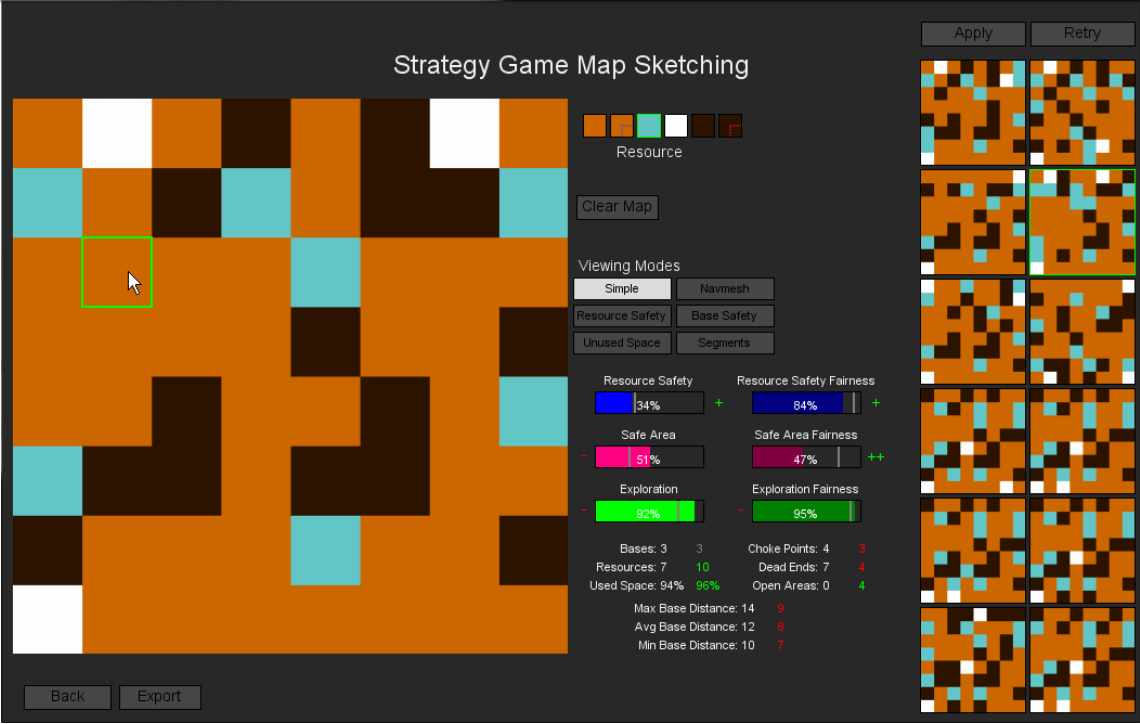
\includegraphics[width=1.0\linewidth]{SentientSketchbook.PNG}
	\caption{Liapis \textit{et al} Sentient Sketchbook during a design session ~\cite{liapis2013sentient}.}
	\label{Sketchbook}
\end{figure} 

\begin{figure}[h]
	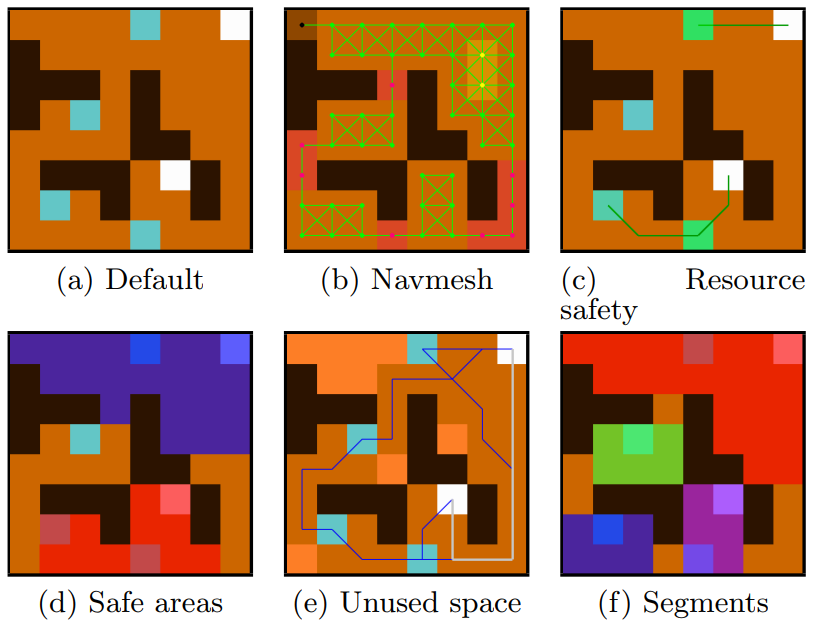
\includegraphics[width=1.0\linewidth]{SentientSketchbook2.PNG}
	\caption{Liapis \textit{et al} Sentient Sketchbook Different viewing modes ~\cite{liapis2013sentient}.}
	\label{Sketchbook2}
\end{figure} 

Baldwin \textit{et al} \cite{baldwin2017mixed} have also implemented a mixed-initiative dungeon designer called the evolutionary dungeon designer or (EDD) for short. EDD is closer to a CAD tool than the IE tool Sentient Sketchbook \cite{liapis2013sentient}.  While the approaches may be different see Figure~\ref{EDD}, both MI tools allow for large customisation of the levels generated see Figure~\ref{EDD}.  Baldwin \textit{et al} \cite{baldwin2017mixed} take a different approach to Liapis  \textit{et al}\cite{liapis2013sentient}.  Baldwin \textit{et al} \cite{baldwin2017mixed} core concept is to identify design patterns within the level design. These design patterns consist of multiple tiles that constitute common patterns found in games. Alvarez \textit{et al}\cite{alvarez2018fostering} builds upon the EDD suggest in \cite{baldwin2017mixed} by adding a IE element to it. It could be argued that the new version of the EDD has an improved interface with lots of its excess drop-down menus gone see Figure~\ref{EDD2}. Beyond the ascetic differences, Alvarez \textit{et al}\cite{alvarez2018fostering} dungeon designer integrates key aspects of  the Sentient Sketchpad \cite{liapis2013sentient}. The second edition of the EDD allows the user to design their own levels, it will then offer suggestions based up the map the user created, this can be seen the top right corner of figure~\ref{EDD2}.  The results from Alvarez \textit{et al}\cite{alvarez2018fostering} experiment focused on whether their tool fostered creativity in the participants using it. Included with the results is a table of requested features made by the participants of the study. One key element highlighted is that the EDD should do a " bit more automated assistance when doing manual designs, which can reduce clicking around the program" \cite[Table 2]{alvarez2018fostering}. Another significant  feature request, was for the dungeon designer to take into account the pattern of the entire dungeon. Using the map of the entire dungeon to generate new rooms.

\begin{figure}[h]
	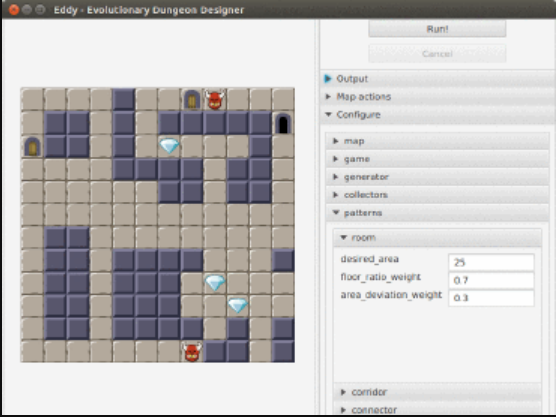
\includegraphics[width=1.0\linewidth]{EDD.PNG}
	\caption{ Baldwin \textit{et al} Evolutionary Dungeon Designer user interface  ~\cite{baldwin2017mixed}.}
	\label{EDD}
\end{figure} 

\begin{figure}[h]
	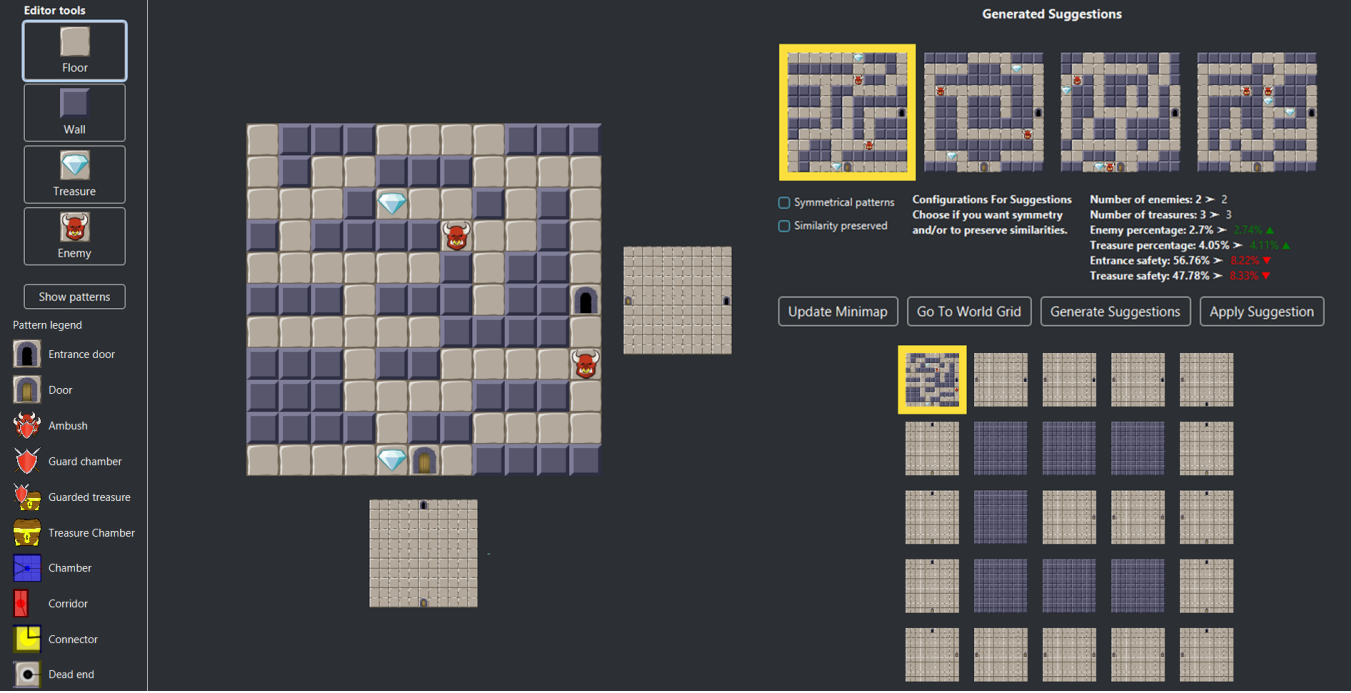
\includegraphics[width=1.0\linewidth]{EDD2.PNG}
	\caption{ Alvarez \textit{et al} Evolutionary Dungeon Designer with modifications user interface  ~\cite{alvarez2018fostering}.}
	\label{EDD2}
\end{figure} 

Horvitz \textit{et al} \cite{horvitz1999principles} propose 12 critical factors to take into consideration when making a mixed-initiative user interface. While Horvitz \textit{et al} \cite{horvitz1999principles}  focuses on a mixed-initiative assistant for Microsoft Outlook (emailing software) it can be argued that some of these factors are relevant for level design.  The first factor that is listed is that an MI tool needs to add significant value through the automation of services. An Examples of a service automated by emailing assistant is the sorting of a user's emails into different categories.   Within in the context of \cite{liapis2013sentient}  they satisfy \cite{horvitz1999principles} first critical factor by allowing the computer to automate some of the map design services like checking for broken game constraints. Liapis \textit{et al} \cite{liapis2013sentient} also allows their algorithm to take on a creative role all be it based on an original human designed map. Within this project, the focus will not be on the creative aspect as the definition of creativity is hard to for a computer to understand \cite{jordanous2010defining}. Alvarez \textit{et al}\cite{alvarez2018fostering} found their MI tool is better at providing controllability than expressivity, when the user imposes their vision, as it is hard for a computer to capture the designers' vision. It can be argued that an MI tool could not consistently add value if it cannot capture the designers' vision. Smith \textit{et al}\cite{smith2011tanagra} believe that human designers strengths lay in creativity and their ability to evaluate good content and the computer lacks this ability. 

Another factor raised by Horvitz \cite{horvitz1999principles} is that a tool must consider minimizing the costs of poor guesses about the users' goals. Even with an extensive history of the users' requirments, a novel use of the tool might be required. It is important for a system to recognise when something novel is happening and for it not to attempt predictions.  Some authors find value in these missed guesses and even seek to find novelty search spaces \cite{liapis2013sentient}. Other authors \cite{liapis2016can,alvarez2018fostering, yannakakis2014mixed} claim these kind of mistakes can foster creativity and alternate suggestions that do not aim to predict the user can be beneficial. On the right-hand side of Figure~\ref{Sketchbook} the results of the guessing algorithm are shown. Clicking retry will remove the current maps and create new ones for the designer to evaluate.

None of the above examples \cite{alvarez2018fostering, liapis2013sentient, baldwin2017mixed} satisfy  Barnes \textit{et al}\cite{barnes2015designing} statement that a mixed-initiative systems UI must provide transparency to the reasoning behind the agents actions. In all cases above\cite{alvarez2018fostering, liapis2013sentient, baldwin2017mixed} , when generating new suggestions the reasoning behind each suggestion was not given to the designer. The designer is presented with the statstics of the current map generated(density, number of resources ETC) but it is not clear from the interface how these statistics are being used. When automating a system transparency is required for a human to trust the automation process \cite{lee2004trust}.

\section{Prediction Methods} \label{prediction}
Predictive texting increases the average message length users send to each other \cite{ling2005length} as well as the speed the words are written \cite{dunlop2000predictive}. The same theory may apply to game design. If patterns to a users game design are established, an AI system may be able to assist in design. In this section, this paper will look into different methods of predicting human requirements, this paper will also discuss the pros and cons of each technique.

The researchers of \cite{chipalkatty2013less} tested alternate methods for predicting human input so as to abstract the low-level movements of the robots the humans were controlling. They built on the idea that humans are good for high-level abstract tasks, but an AI agent was much better at performing low-level repetitive control tasks. In addition, they found that when trying to predict the next human input, trying to identify patterns in a history of events was not successful. Instead, using just the last event yielded much better results, hence their title "less is more". Instead of using current human inputs, \cite{bhatia2016targeted} used the history of the users' social media page to predict the users' interests. Perhaps if the authors of \cite{chipalkatty2013less} had looked less at the input history of the human and instead focused on grouping inputs together to create larger actions. Similar, to how modern day phones often predict entire sentences rather than just single words.

\subsection{Markov Chains}
Markov Chains is a theory similar to the most successful method found by Bhatia\textit{et al} \cite{bhatia2016targeted}. A Markov chain is a special kind of process that works under the assumption that the state at time \textit{t+1} depends only on the current state. To put it another way, the state at time \textit{t+1} is exclusively dependent on the state at time \textit{t}. This means State \textit{t+1}  is not dependent on the history of the states leading up to it\cite{ye2000markov}. While this technique may be useful for predicting anomalies in systems \cite{ju2001hybrid, gwadera2005markov, ye2000markov} where the states are heavily dependent on the latter state happening. It is hard to see how during a creative process where the next state is dependent on the vision of the design state \textit{t+1} can be predicted just from knowing state \textit{t}. The introduction of a Markov model makes this method more viable. A Markov model can be used to describe the probabilistic relationship between the previous states in a Markov Chain\cite{markov1971extension}.  Higher order Markov chains relax the rule of the next state being only dependent on the current state by allowing the network structure to look \textit{n} number of states back from the current state\cite{ching2008higher}. Snodgrass \textit{et al}\cite{snodgrass2017learning}used Markov models as a way to model level data  .Using these Markov models Snodgrass \textit{et al}\cite{snodgrass2017learning} applied different sampling techniques, they found using their higher order Markov chains were more effective than using just Markov chains.  This conflicts with Chipalkatty \textit{et al}\cite{chipalkatty2013less} findings of "less is more", Snodgrass \textit{et al}\cite{snodgrass2017learning} found that using a history of states to predict the next state was more effective to achieve their goals.

\subsection{Artifical Neural Network}
An artificial neural network (ANN) consists of many nodes that are divided into separate layers. Each node receives inputs from other nodes, the value of these inputs depends on the weight of the connection between the nodes \cite{lai2010prediction}. ANN are used in prediction methods focusing on outputting numerical values \cite{lai2010prediction, akdag2009estimation}. Shepperd \textit{et al} \cite{shepperd2001comparing} found that case-based reasoning(CBR) outperformed a ANN on more occasions. However, Shepperd \textit{et al}\cite{shepperd2001comparing} highlighted the dependence of the respective techniques on the nature of the training sets used. Figure~\ref{learningSets} shows a stepwise regression procedure proving to be more accurate at prediction than both CBR and ANN on small datasets.  A time series approach to neural networks has been found to increase their accuracy when dealing with world state predictions \cite{hazarika1998neural}. Although the training set Hazarika \textit{et al} used was the large number at 500 data points for training and 250 points for validation. Looking at examples from \cite{liapis2013sentient, alvarez2018fostering,  baldwin2017mixed} the maximum levels sizes are 12 wide by 12 tall. This means that the maximum number of data points provided by one map would be 124, which is far less than Hazarika \textit{et al} use to train their ANN.

\begin{figure}[h]
	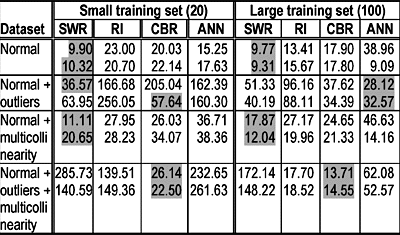
\includegraphics[width=1.0\linewidth]{trainingSets.PNG}
	\caption{Shepperd \textit{et al}  Analysis of Accuracy (MMRE) for Continuous Model (Y1)  ~\cite{shepperd2001comparing}.}
	\label{learningSets}
\end{figure} 

\subsection{Stepwise Regression Procedure}

\section{Methodology}
One of the key motivators for this experiment comes from Alverezs' \textit{et al}\cite{alvarez2018fostering} literature, in particular a users' feature request for more automated assistance to reduce clicking. To this end, this project proposes a tile based level editor which has a mixed-initiative component. The mixed-initiative component will reduce clicks by predicting what the users next action will be. In addition, this level design tool will be used to discover if the predictive texting findings of Ling \cite{ling2005length}  and Dunlop \textit{et al}\cite{dunlop2000predictive} are applicable to level design. The research question proposed in this project is: How Will a Mixed-Initiative Level Designer that Predicts User Requirements Affect the Levels Created? 

\subsection{Hypothesis}\label{hypothesis}
When creating a level designer the aim is to always increase the ease at which levels could normally be created. For the scope of this paper, the hypothesises will focus on MI tool within the context of the editor, not the editor itself. Table ~\ref{hyp} shows the hypothesises researched in this paper, it also shows from which source of data each hypothesis depends. Hypothesises 2 and 1 will be addressing  Ling \cite{ling2005length}  and Dunlop \textit{et al}\cite{dunlop2000predictive} predictive texting results and whether they will also prove true in a level editor. Hypothesis 3 will be investigating whether a predictive tool will satisfy the feature proposed by  Alverezs' \textit{et al}\cite{alvarez2018fostering}. Hypothesis 4 will build on the work of  Alvarez' \textit{et al}\cite{alvarez2018fostering} and see if an MI level designer can make designers consider alternative level design approaches. Finally, hypothesis 5 will discover if designers with more experience are more likely to find the MI a negative influence than designers with less experience.

\begin{table*}[h]
		\centering
		\caption{Hypothesis Table}
		\label{hyp}
		\def\arraystretch{1.5}
		\begin{tabular}{|c|p{7cm}|p{7cm}|p{1.75cm}|}
			\hline
			& \textbf{Hypothesis}& \textbf{Null Hypothesis} & \textbf{Data Source}\\\hline
			1 & The MI tool will effect the speed at which the participants create levels.
			& The MI tool will not effect the speed at which the participants create levels.
			& Design Session Statistics\\ \hline
			
			2 & The MI tool will effect the size of the levels the participants create.
			&  The MI tool will not effect the size of the levels the participants create.
			& Design Session Statistics\\ \hline

			3 & The MI tool will effect the number of the clicks the designer makes.
			&  The MI tool will not effect the number of the clicks the designer makes.
			& Design Session Statistics\\ \hline

			4 & The MI tool will influence participants to explore other level designs.
			& The MI tool wil not influence participants to explore other level designs.
			&  Questionnaire\\ \hline

		          5 & The participants with more experience will be Negatively impacted more often by the MI tool.
			&  There will be no correlation between experience and the negative impact of the MI tool.
			& Questionnaire\\ \hline
			
		\end{tabular}
\end{table*}

\subsection{Participants}
The participants for this experiment will be randomly sampled from Falmouth University Games Academy. As such, most participants will have some game design experience experience. A power analysis for this experiment resulted in a sample sixe of 23.  In this experiment all of the participants will be in one group, they will each be required to design levels using the level editor provided. By the end of the experiment, all of the participants will have designed the same number of levels. Everyone in this study will be given a consent form, an information sheet and the option to quit the experiment at any time. The information sheet will only give the basic information of the project as we do not want to invite acquiescence bias\cite{watson1992correcting}. The data collected in this experiment will not be enough to identify anyone, keeping the participants anonymity safe.

\subsection{Design Session}
The design session will require the participants to create five different levels each with different editor settings. Before the session starts the users are prompted with a multiple choice question. This question will enquire into the participants' game design experience, measured in years. The user will be presented with the main level designer interface. They will have up to one minute to familiarise themselves with the interface before the experiments start. The different editor settings the participants will be working in can be seen in Table~\ref{settings}. The order in which the different settings will occur will be random, this will reduce the impact of the practice effect on any data gathered. The computer will choose the order in which the editor setting will be applied. This means the observing researcher will not know what current settings are applied.  Making this a double-blind study which will stop investigator/observer bias \cite{phillips1999double}. Before each level starts an on-screen prompt will inform the user of the rules of the current level, for example: "This level has a max size of 24 x 24 tiles.". After completion of each level, the designer will be asked four multiple choice questions.  Each question will have five possible answers, the answers are relative to the questions asked. After the questions have been answered the answers, the map settings, the time is taken and a layout of the map will all be saved.
 The questions are:
\begin{itemize}
    \item How frequently did the level designer make you consider an alternative level design?
    
    \item How much impact did the level designer have on your work flow?

    \item What kind of impact did the level designer have on your work flow?
\end{itemize}
An alternate method would be to have a questionnaire at the end of the experiment once all levels have been completed. However, as each set of responses correlates to a level for data management having being directly associated with the level is easier. In addition, leaving the questions until the end in one questionnaire may invite levelling and sharpening bias, this is where details are lost and other are heightened over time \cite{koriat2000toward}.

\begin{table}[h]
	\centering
	\caption{Editor Settings}
	\label{settings}
	\def\arraystretch{2}
\resizebox{\columnwidth}{!}{\begin{tabular}{|l|l|l|l|l|}
		\hline
		\textbf{Editor Settings} & \textbf{Predictive Placements Enables}& \textbf{Unrestricted size } & \textbf{Exploration}\\\hline
		Settings 1  &  X & X& \\ \hline
		Settings 2  &     & X &\\ \hline
		Settings 3  &   X&  &\\ \hline
		Settings 4  &    &  &\\ \hline
		Settings 5  & X &   & X\\ \hline
	\end{tabular}}
\end{table}

\bibliographystyle{IEEEtran}
\bibliography{references}

% Appendices

\appendices
\section{First appendix}
Appendices are optional. Delete or comment out this part if you do not need them.

% that's all folks
\end{document}
